
    \centering
    \tikzsetnextfilename{conj_elemental3_R3}
    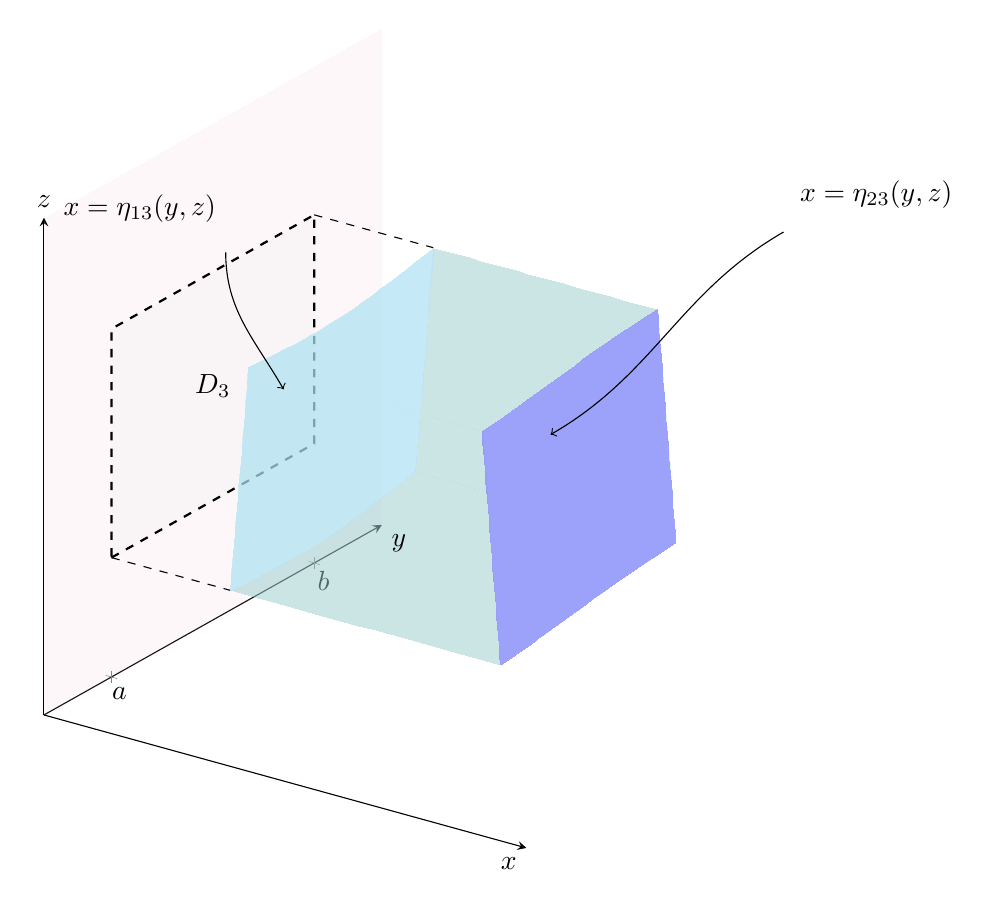
\begin{tikzpicture}
    \begin{axis}[
        view={35}{25}, 
        width=12cm, height=12cm,
        grid=none,
        axis lines=center,
        xmin=0, xmax=6, % Eje de proyección x
        ymin=0, ymax=5,
        zmin=0, zmax=5,
        xtick=\empty, ytick={1,4}, yticklabels={$a$,$b$},
        ztick=\empty,
        xlabel={$x$}, ylabel={$y$}, zlabel={$z$},
        every axis x label/.style={at={(ticklabel* cs:1)},anchor=north east},
        every axis y label/.style={at={(ticklabel* cs:1)},anchor=north west},
        every axis z label/.style={at={(ticklabel* cs:1)},anchor=south},
        clip=false
    ]

    % --- 0. Plano de fondo Lila (yz en x=0) ---
    \addplot3 [surf, domain=0:5, domain y=0:5, samples=2, opacity=0.1, colormap={lila}{color=(purple!30) color=(purple!30)}, shader=interp, draw=none] (0,x,y);

    % --- 1. Dominio D_3 en R2 (Plano yz) ---
    \addplot3 [surf, domain=1:4, domain y=1.2:3.5, samples=2, opacity=0.15, colormap={gray}{color=(gray!20) color=(gray!20)}, shader=interp, draw=none] 
        (0, x, y);
    \draw[dashed, black, thick] (0, 1, 1.2) -- (0, 4, 1.2) -- (0, 4, 3.5) -- (0, 1, 3.5) -- cycle;

    % --- 2. Paredes del volumen (Relleno completo de las 4 caras laterales) ---
    % Pared superior en z = 3.5
    \addplot3 [surf, domain=1:4, domain y=0:1, samples=20, opacity=0.3, colormap={teal}{color=(teal!40) color=(teal!40)}, shader=interp, draw=none] 
        ({ (1-y)*(1.2 + 0.2*sin(x*50) + 0.1*3.5) + y*(4.8 + 0.2*cos(x*40) - 0.1*3.5) }, x, 3.5);
    
    % Pared inferior en z = 1.2
    \addplot3 [surf, domain=1:4, domain y=0:1, samples=20, opacity=0.3, colormap={teal}{color=(teal!40) color=(teal!40)}, shader=interp, draw=none] 
        ({ (1-y)*(1.2 + 0.2*sin(x*50) + 0.1*1.2) + y*(4.8 + 0.2*cos(x*40) - 0.1*1.2) }, x, 1.2);

    % Pared lateral anterior en y = 1 (Une de z=1.2 a z=3.5)
    \addplot3 [surf, domain=1.2:3.5, domain y=0:1, samples=20, opacity=0.3, colormap={teal}{color=(teal!40) color=(teal!40)}, shader=interp, draw=none] 
        ({ (1-y)*(1.2 + 0.2*sin(1*50) + 0.1*x) + y*(4.8 + 0.2*cos(1*40) - 0.1*x) }, 1, x);

    % Pared lateral posterior en y = 4 (Une de z=1.2 a z=3.5)
    \addplot3 [surf, domain=1.2:3.5, domain y=0:1, samples=20, opacity=0.3, colormap={teal}{color=(teal!40) color=(teal!40)}, shader=interp, draw=none] 
        ({ (1-y)*(1.2 + 0.2*sin(4*50) + 0.1*x) + y*(4.8 + 0.2*cos(4*40) - 0.1*x) }, 4, x);

    % --- 3. Superficie Trasera x = eta13 ---
    \addplot3 [surf, domain=1:4, domain y=1.2:3.5, samples=25, opacity=0.6, colormap={cyan}{color=(cyan!30) color=(cyan!30)}, shader=interp, draw=none] 
        ({ 1.2 + 0.2*sin(x*50) + 0.1*y }, x, y);

    % --- 4. Superficie Delantera x = eta23 ---
    \addplot3 [surf, domain=1:4, domain y=1.2:3.5, samples=25, opacity=0.7, colormap={blue}{color=(blue!50) color=(blue!50)}, shader=interp, draw=none] 
        ({ 4.8 + 0.2*cos(x*40) - 0.1*y }, x, y);

    % --- 5. Proyecciones punteadas al plano ---
    \draw[dashed, thin] (0,1,1.2) -- ({1.2+0.2*sin(50)+0.1*1.2}, 1, 1.2);
    \draw[dashed, thin] (0,4,3.5) -- ({1.2+0.2*sin(200)+0.1*3.5}, 4, 3.5);

    % --- 6. Etiquetas y flechas optimizadas ---
    \node at (0, 2.5, 2.35) {$D_3$};
    
    % Flecha para la sábana frontal (azul)
    \node[anchor=south west] at (5.5, 4.5, 4.5) {$x = \eta_{23}(y,z)$};
    \draw[->, thin] (5.5, 4.4, 4.4) to[out=210, in=30] (4.2, 2.5, 2.8);
    
    % Flecha para la sábana trasera (cyan) - Desde arriba apuntando hacia abajo
    \node[anchor=south east] at (1.0, 1.5, 4.5) {$x = \eta_{13}(y,z)$};
    \draw[->, thin] (1.0, 1.5, 4.3) to[out=270, in=120] (1.3, 2.0, 2.8);

\end{axis}
\end{tikzpicture}
\caption{Conjunto elemental de Tipo 3.}
